\chapter{Implications for CHIPS}
\label{chap:implications}

\section{Alternative implementations} %%%%%%%%%%%%%%%%%%%%%%%%%%%%%%%%%%%%%%%%%%%%%%%%%%%%%%%%%%%%
\label{sec:cvn_alt} %%%%%%%%%%%%%%%%%%%%%%%%%%%%%%%%%%%%%%%%%%%%%%%%%%%%%%%%%%%%%%%%%%%%%%%%%%%%%%

The work outlined in this chapter is the result of extensive testing and optimisation of many
differing approaches to applying CNNs to \chips. Here we highlight some interesting findings from
this process to both provide completeness, but also to hopefully inform future work on this topic.

\subsubsection*{Alternative inputs} %%%%%%%%%%%%%%%%%%%%%%%%%%%%%%%%%%%%%%%%%%%%%%%%%%%%%%%%%%%%%%

There are many possible event representations that can be used as input to the CNNs in this work.
Three different approaches are explored in this work!

- New ideas with x+ x- mapping in Ref.~\cite{berns2020}
- Fraction of deposited charge in endcaps = 0.4769380479133997

\begin{equation} % ISO CASE EQUATION %
    X_{\pm}=
    \begin{cases}
        1-\chi_{\mp} & (z \geq 0) \\
        \chi_{\pm}   & (z < 0)
    \end{cases}
    \label{eq:iso_case}
\end{equation}

\begin{equation} % ISO MAIN EQUATION %
    \chi_{\pm}=W(\rho,z)\frac{\pi\pm\phi}{2\pi}
    \label{eq:iso_main}
\end{equation}

\begin{equation} % ISO PART EQUATION %
    W(\rho,z)=\sqrt{\frac{\rho^{2}-2R|z|+RH}{R^{2}+RH}}
    \label{eq:iso_part}
\end{equation}

- where R and Z are the radius and height of the detector cylinder and W is chosen for constant
surface density.
- Turns out removing the distortions of not viewing the event from the vertex is the most
important thing!!!

- Approaches in the past for event classification using CNNs for water cherenkov detectors have
taken a few Approaches to generating the input image representation.
- Projecting onto a 2d surface "outside" the detector

\begin{table}
    \begin{tabular}{cccc}
        Metric                   & Vertex View & Origin Raw View & Origin Iso View \\
        \midrule
        Maximum FOM              & 0.461       & 0.422           & 0.419           \\
        Highest Score Efficiency & 0.878       & 0.874           & 0.867           \\
        Highest Score Purity     & 0.354       & 0.291           & 0.298           \\
        ROC Integral             & 0.825       & 0.822           & 0.821           \\
        PRC Integral             & 0.707       & 0.675           & 0.670           \\
    \end{tabular}
    \caption[Comparison of performance metrics for three input image representations.]
    {Comparison of performance metrics for the three input image representations considered. The
        highest score selection uses the highest scoring output neuron for classification. The ROC
        and PRC integrals are taken from the curves shown in
        Fig.~\ref{fig:repr_nuel_comp_curves}.}
    \label{tab:repr}
\end{table}

\begin{figure} % REPR NUEL EFF CURVES DIAGRAM %
    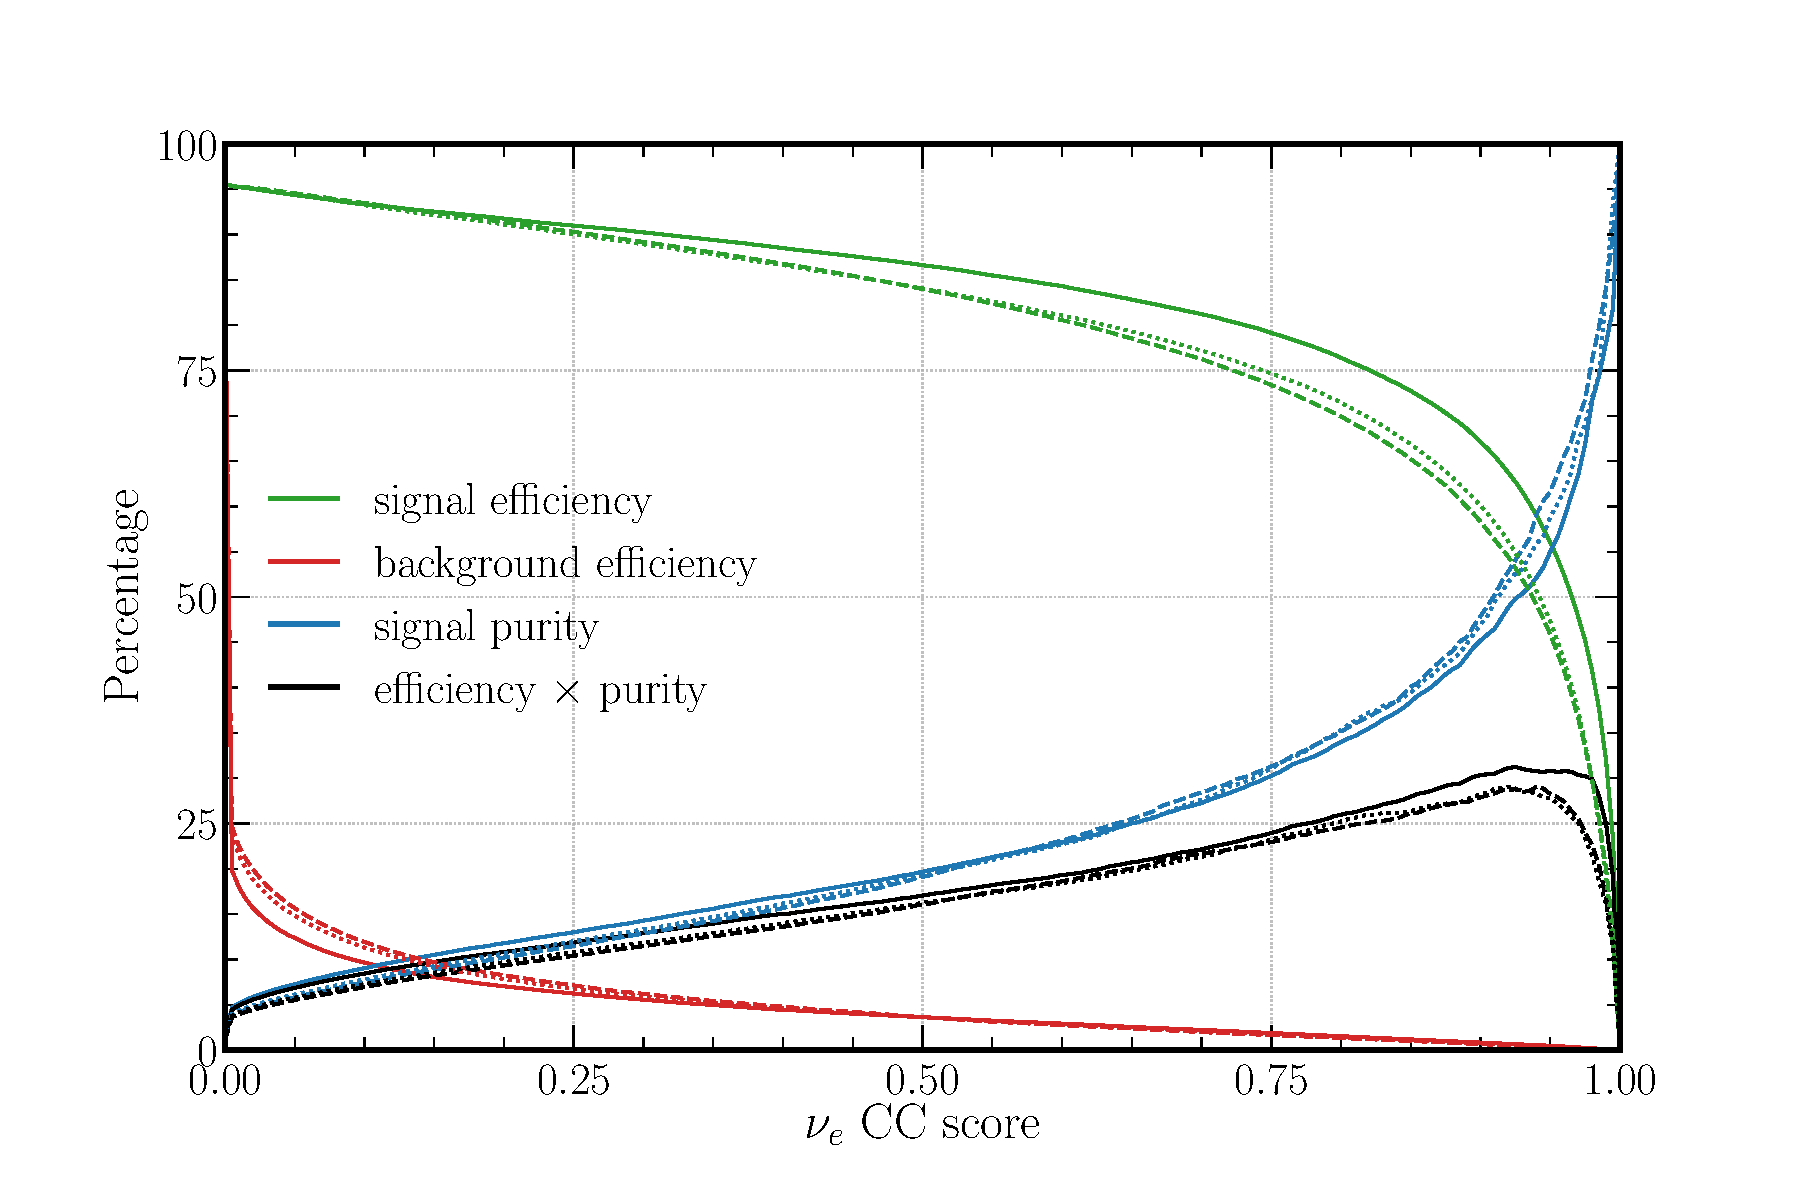
\includegraphics[width=0.7\textwidth]{diagrams/6-cvn/chipsnet/repr_nuel_eff_curves.pdf}
    \caption[CC $\nu_{e}$ efficiency and purity curves for the three input image representations.]
    {CC $\nu_{e}$ efficiency, purity and $\mathrm{efficiency}\times\mathrm{purity}$ for different
        values of CC $\nu_{e}$ score selection for the three input image representations
        considered. The \emph{vertex view} curves are shown by the solid lines, the \emph{origin
            raw view} curves by the dashed lines, and the \emph{origin dotted} surves by the dotted
        lines.}
    \label{fig:repr_nuel_eff_curves}
\end{figure}

\begin{figure} % REPR NUEL COMP CURVES DIAGRAM %
    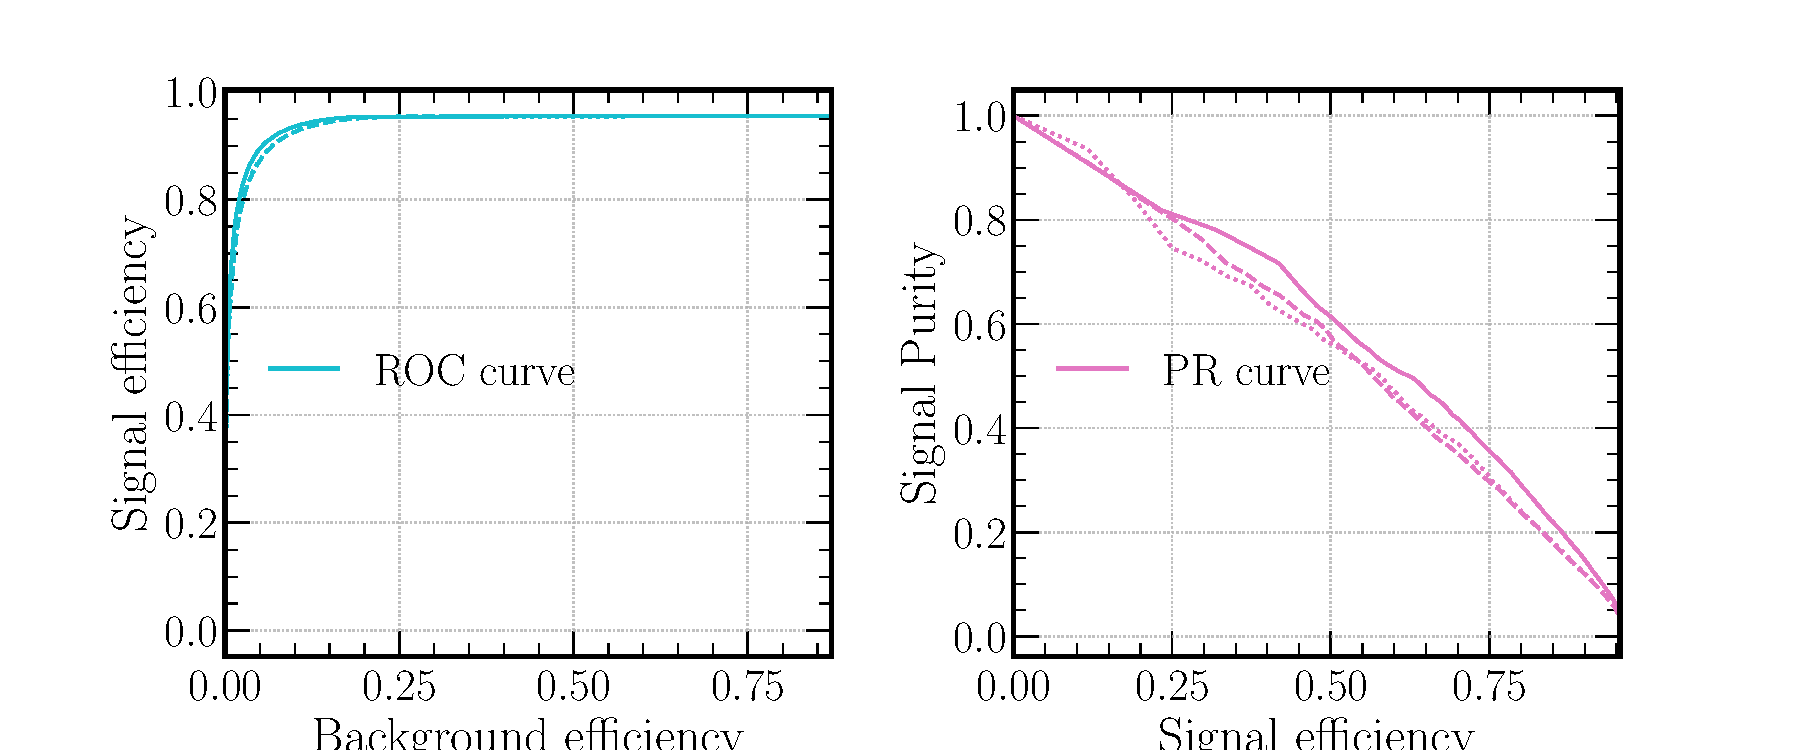
\includegraphics[width=0.8\textwidth]{diagrams/6-cvn/chipsnet/repr_nuel_comp_curves.pdf}
    \caption[Comparison curves for the three input image representations considered.]
    {Comparison curves for the three input image representations considered. Signal vs background
        selection efficiencies as the CC $\nu_{e}$ score selection is varied (left). Signal CC
        $\nu_{e}$ purity vs efficiency as the CC $\nu_{e}$ score selection is varied (right). The
        \emph{vertex view} curves are shown by the solid lines, the \emph{origin raw view} curves
        by the dashed lines, and the \emph{origin dotted} curves by the dotted lines. The left
        plot contains what are commonly referred to as receiver-operator curves (ROC), while the
        right plot contains precision-recall (PRC) curves.}
    \label{fig:repr_nuel_comp_curves}
\end{figure}

\begin{table}
    \begin{tabular}{cccc}
        Metric                   & Charge & Charge+Time & Charge+Time+Hough \\
        \midrule
        Maximum FOM              & 0.436  & 0.461       & 0.465             \\
        Highest Score Efficiency & 0.869  & 0.878       & 0.877             \\
        Highest Score Purity     & 0.357  & 0.354       & 0.369             \\
        ROC Integral             & 0.824  & 0.825       & 0.826             \\
        PRC Integral             & 0.689  & 0.707       & 0.712             \\
    \end{tabular}
    \caption[Comparison of performance metrics for each additional input image map.]
    {Comparison of performance metrics for each additional input image map. The highest score
        selection uses the highest scoring output neuron for classification.}
    \label{tab:chan}
\end{table}

\subsubsection*{Alternative training samples} %%%%%%%%%%%%%%%%%%%%%%%%%%%%%%%%%%%%%%%%%%%%%%%%%%%%

\begin{figure} % REPR NUEL EFF CURVES DIAGRAM %
    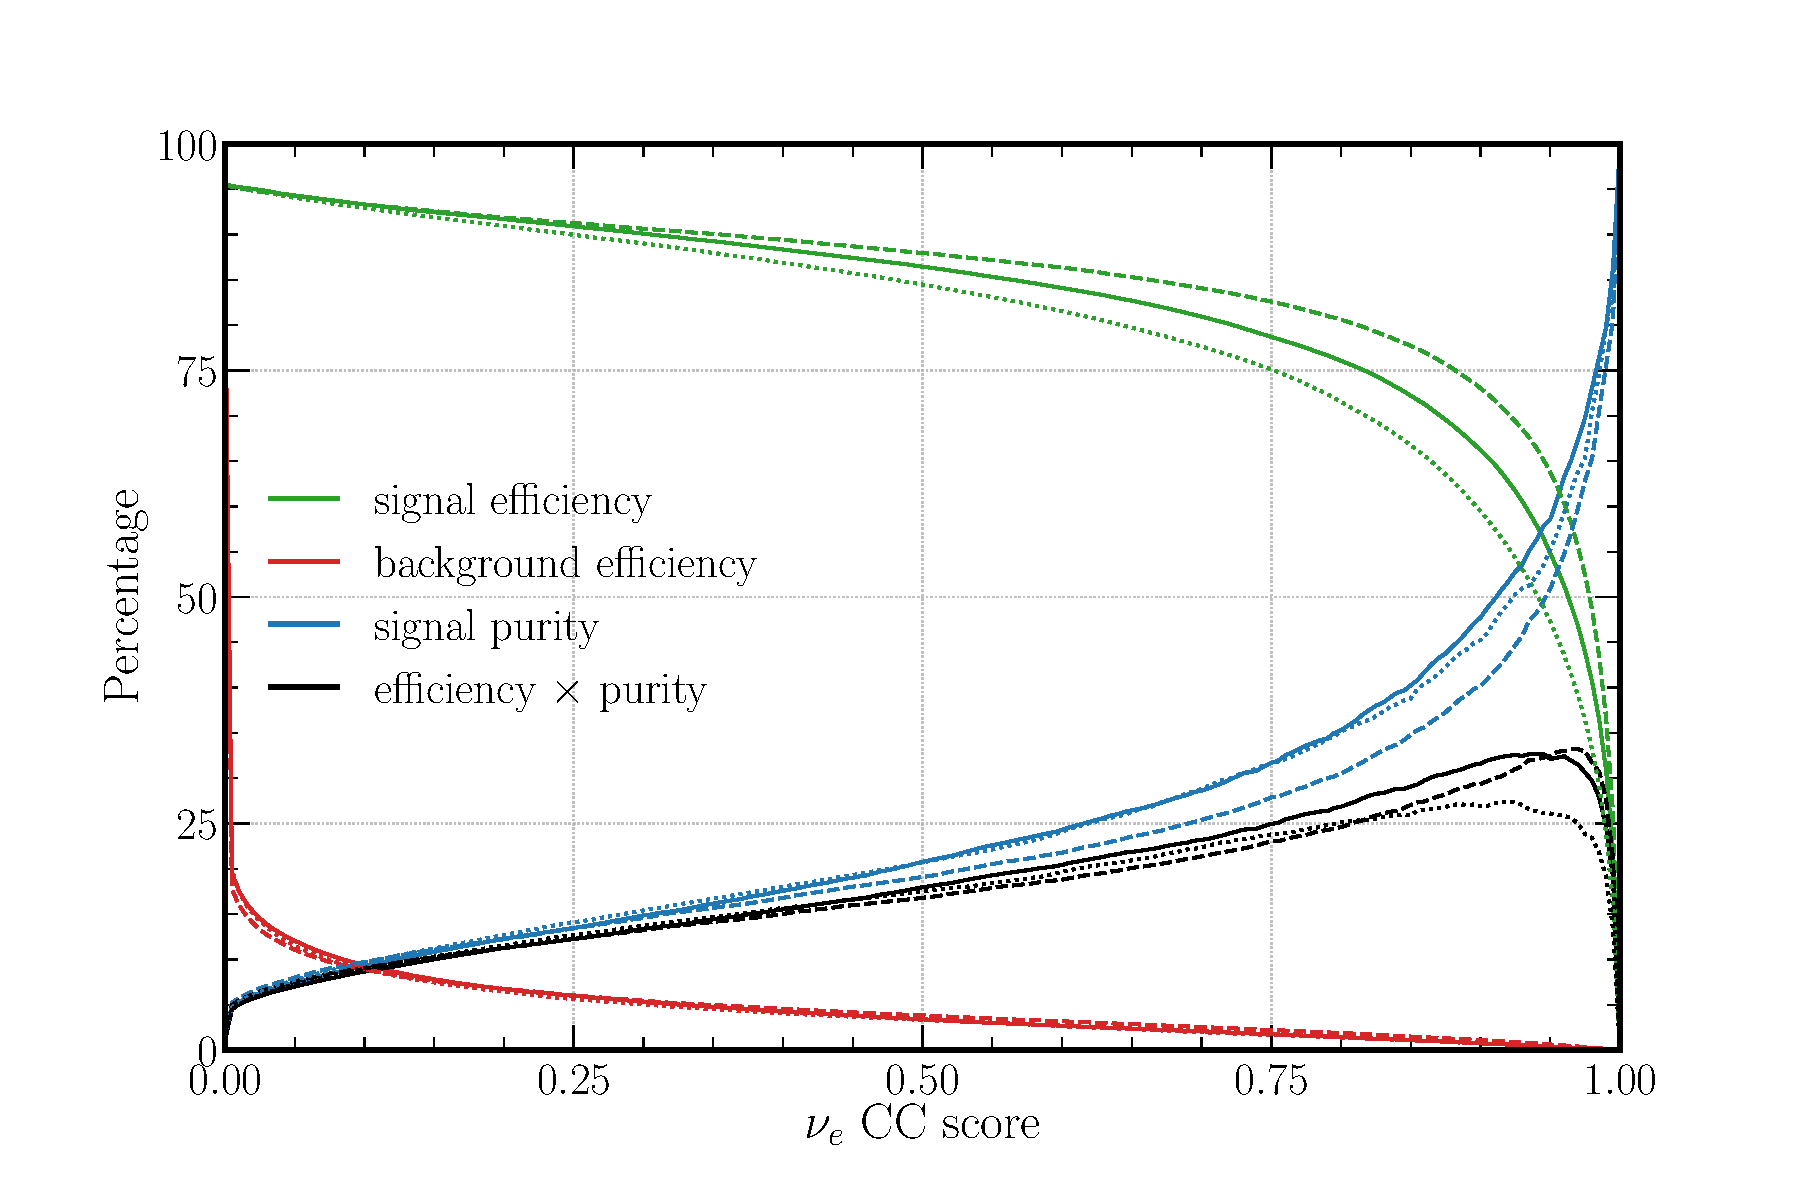
\includegraphics[width=0.7\textwidth]{diagrams/6-cvn/chipsnet/sample_nuel_eff_curves.pdf}
    \caption[CC $\nu_{e}$ efficiency and purity curves for the different training samples.]
    {CC $\nu_{e}$ efficiency, purity and $\mathrm{efficiency}\times\mathrm{purity}$ for different
        values of CC $\nu_{e}$ score selection for the different training samples considered. The
        \emph{vertex view} curves are shown by the solid lines, the \emph{origin raw view} curves
        by the dashed lines, and the \emph{origin dotted} surves by the dotted lines.}
    \label{fig:sample_nuel_eff_curves}
\end{figure}

\begin{figure} % REPR NUEL COMP CURVES DIAGRAM %
    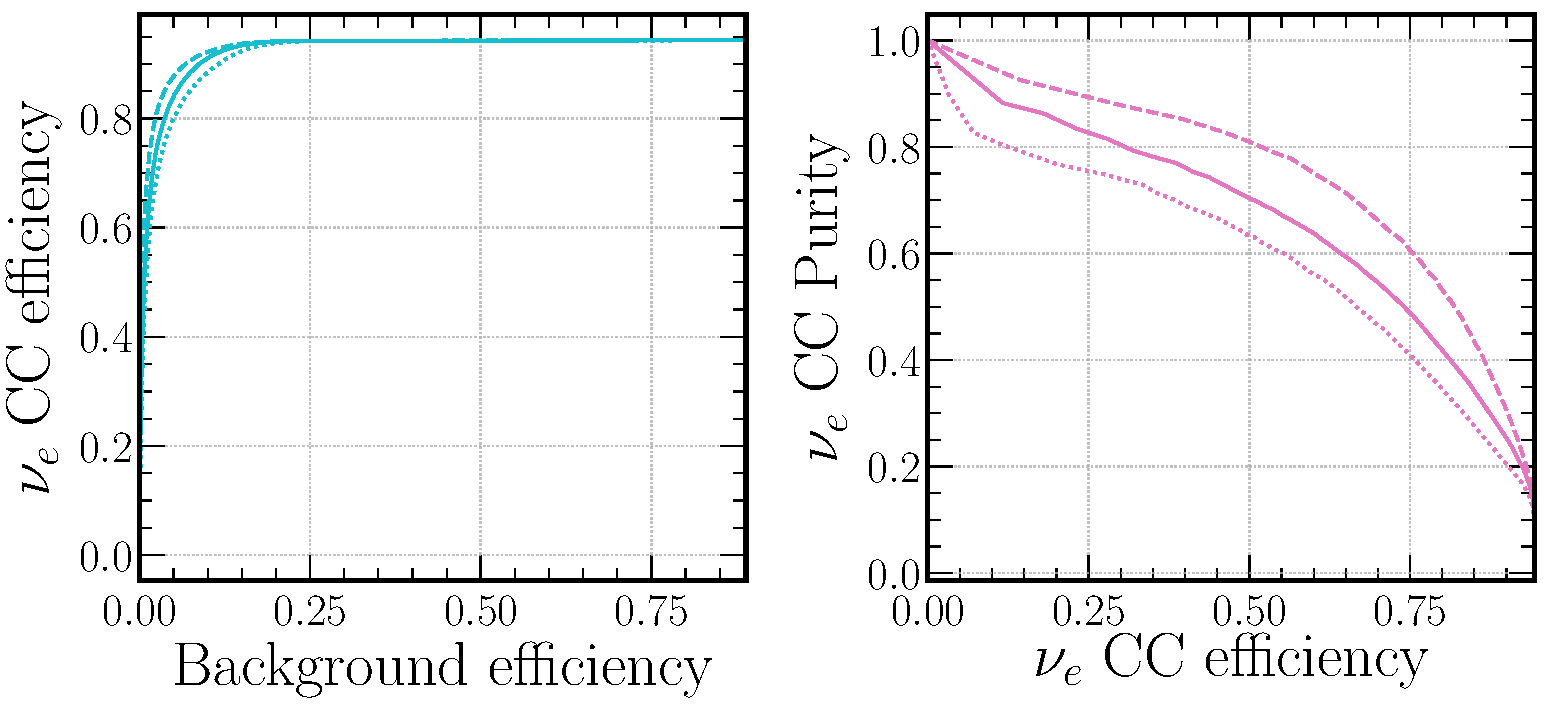
\includegraphics[width=0.8\textwidth]{diagrams/6-cvn/chipsnet/sample_nuel_comp_curves.pdf}
    \caption[Comparison curves for the different training samples considered.]
    {Comparison curves for the different training samples considered. Signal vs background
        selection efficiencies as the CC $\nu_{e}$ score selection is varied (left). Signal CC
        $\nu_{e}$ purity vs efficiency as the CC $\nu_{e}$ score selection is varied (right). The
        \emph{flux+uniform} curves are shown by the solid lines, the \emph{flux} curves by the
        dashed lines, and the \emph{uniform} curves by the dotted lines. The left plot contains
        what are commonly referred to as receiver-operator curves (ROC), while the right plot
        contains precision-recall (PRC) curves.}
    \label{fig:sample_nuel_comp_curves}
\end{figure}

\begin{table}
    \begin{tabular}{cccc}
        Metric                   & Flux  & Uniform & Flux+Uniform \\
        \midrule
        Maximum FOM              & 0.465 & 0.339   & 0.386        \\
        Highest Score Efficiency & 0.877 & 0.799   & 0.834        \\
        Highest Score Purity     & 0.369 & 0.347   & 0.368        \\
        ROC Integral             & 0.826 & 0.815   & 0.820        \\
        PRC Integral             & 0.712 & 0.568   & 0.634        \\
    \end{tabular}
    \caption[Comparison of performance metrics for the different training samples considered.]
    {Comparison of performance metrics for the different training samples considered. The highest
        score selection uses the highest scoring output neuron for classification.}
    \label{tab:sample}
\end{table}

\subsubsection*{Alternative architectures} %%%%%%%%%%%%%%%%%%%%%%%%%%%%%%%%%%%%%%%%%%%%%%%%%%%%%%%

- truncated versions of the other networks so they have approximately the same number of
parameters to train for making a good comparison.

\begin{table}
    \begin{tabular}{ccccc}
        Metric                   & VGG        & Inception  & ResNet     & Inception-ResNet \\
        \midrule
        Number of parameters     & 17,225,296 & 16,893,216 & 16,526,288 & 17,145,238       \\
        Iteration time (ms)      & 88         & 192        & 112        & 209              \\
        Maximum FOM              & 0.465      & 0.459      & 0.445      & 0.444            \\
        Highest Score Efficiency & 0.877      & 0.870      & 0.869      & 0.874            \\
        Highest Score Purity     & 0.369      & 0.373      & 0.374      & 0.349            \\
        ROC Integral             & 0.825      & 0.825      & 0.824      & 0.824            \\
        PRC Integral             & 0.712      & 0.706      & 0.688      & 0.699            \\
    \end{tabular}
    \caption[Comparison of performance metrics for the different network architectures considered.]
    {Comparison of performance metrics the different network architectures considered. The highest
        score selection uses the highest scoring output neuron for classification.}
    \label{tab:arch}
\end{table}

\subsubsection*{Alternative beam categorisation} %%%%%%%%%%%%%%%%%%%%%%%%%%%%%%%%%%%%%%%%%%%%%%%%%

- The choice of categorisation can matter
- All categories CC QE, Res, DIS, Coh, MEC, and other for both $\nu_{e}$ and $\nu_{\mu}$, plus NC
Res, DIS, Coh, and other, for a total of 16 categories. You can then sum the scores as Nova have
done etc.... to get the combined categories
- Fully combined, you may think would work better as it just focuses on what we want to optimise.
This is CC $\nu_{e}$, CC $\nu_{\mu}$, and NC.
- Combined plus the CC and NC cats that are masked like in this work described above.

\begin{table}
    \begin{tabular}{cccc}
        Metric                   & All   & Full-Comb & Multi (learnt) \\
        \midrule
        Maximum FOM              & 0.465 & 0.451     & 0.471          \\
        Highest Score Efficiency & 0.877 & 0.871     & 0.872          \\
        Highest Score Purity     & 0.369 & 0.359     & 0.392          \\
        ROC Integral             & 0.826 & 0.825     & 0.826          \\
        PRC Integral             & 0.712 & 0.692     & 0.716          \\
    \end{tabular}
    \caption[Comparison of performance metrics for the different beam categorisations considered.]
    {Comparison of performance metrics for the different beam categorisations considered. The highest
        score selection uses the highest scoring output neuron for classification.}
    \label{tab:cat}
\end{table}


\begin{comment}
CALIBRATION SENSITIVITY
TROUBLESOME EVENTS
PMT DISTRIBUTION
TIMING RESOLUTION
WATER QUALITY
POSSIBLE IMPROVEMENTS

- You have all of these possible parameters that can affect the performance (event categorisation
and kinematic reconstruction) of your WC detector

- Positioning of the detector (L, angle off-axis, overburden) *
- Size of the detector (height and radius) *
- Water quality (attenuation length, scattering vs absorption) *
- Which PMT’s you use (time resolution, charge collection) *
- How the PMT’s are positioned (percentage coverage, zones)
- Calibration quality (position, time, charge)
- Reconstruction methodology (likelihood vs CNN)
- Given these restrictions

- Only certain mine pits usable (fixes L and angle off-axis, use all overburden available)
- 12.5m radius for practical construction (fixes radius, but not height)
- Want to be able to carry the planes easily (Adds limits to PMT coverage percentage)
- Will just be looking at beam events, should not need much in the back
- PMT’s available. Due to cost etc… we fix the PMT’s we use, can still explore this space with
varying the time/charge. Can look at
\end{comment}

- but was mainly chosen to speed up iteration of network optimisation.
- This works out at 2.5m is theta and 2m in phi approx (when viewed from the centre of the detector)